\section{Abstract}

In this report, three image classification model variants trained on the same coffee leaf disease
dataset were compared. The objective of this study was to classify images of coffee leaves
into one of three classes -- healthy leaves, coffee leaf rust, and Phoma disease. The
models tested in this experiment were a baseline MobileNetV2 transfer learning model, a
MobileNetV2 model with a denser classifier head, and a Simple CNN. All models used the
same training, validation, and testing folders, the same batch size, and input images of
224 x 224 pixels. The three output classes for both MobileNetV2 versions and the Simple
CNN were the same as well. After the additional experiment, the MobileNetV2 dense-head
model performed best, achieving 97.53\% test accuracy, compared with 94.23\% for the
MobileNetV2 baseline and 95.88\% for the Simple CNN. However, the improved MobileNetV2
result was obtained by increasing the trainable capacity of the classifier head.

\section{Introduction}

Coffee leaf diseases may decrease crop productivity and quality. Machine vision-based
computer models can assist farmers with automated disease detection by learning from
labeled images of healthy and diseased leaves. In the current project, the task was not only to build a
model that performed classification accurately, but also to compare different methods and
analyze the differences between the chosen models. Such analysis was useful since the
model with the best accuracy was not necessarily the most efficient one to deploy. In this
paper, the criteria for comparison included such parameters as accuracy, loss, performance
per class, the number of model parameters, preprocessing, limitations and possible
problems with the dataset.

The models discussed in this experiment belonged to two widely-used types of image
classification techniques. The first approach used transfer learning based on pre-trained
MobileNetV2. Two classifier heads were tested while the remaining feature extraction part
of the model was kept frozen. The second approach used a custom CNN architecture which
learned convolutional filters during the training process using the dataset. These models
were applied depending on the conditions: transfer learning in case there was a lack of
labeled data and training from scratch when the available dataset was sufficient.

\subsection{Related Work and Scientific Context}

Previous works demonstrate that accurate plant disease image classification could be
accomplished if both training and validation images come from the same data set;
however, it is not always the case. Mohanty et al. trained their deep learning
algorithm on the PlantVillage data set and obtained 99.35\% classification accuracy.
Nonetheless, when their model was trained using other online images, the overall
accuracy reached just 31.4\%. It follows that although high accuracy within the same
data set demonstrates feasibility, it still should not be considered a sufficient
condition for deployment \cite{Mohanty2016}.

This applies even for more specialized models designed to recognize coffee-related
diseases. Esgario et al. used CNN-based classifiers to distinguish different coffee
biotic stresses and their severity. The authors obtained 95.24\% accuracy for
classification and 86.51\% for estimation of coffee leaves' disease severity
\cite{Esgario2020}. In this paper, the authors also noted that some errors occurred due
to the resemblance of the disease's signs and due to imbalanced dataset. Consequently,
failure cases in scientific studies provide information about the limitations of the
approach and necessary improvements.

Several specific coffee leaf data sets, such as RoCoLe and JMuBEN/JMuBEN2, have been
developed recently to improve image availability. RoCoLe contains Robusta coffee leaf
images, while JMuBEN and JMuBEN2 include 58,555 Arabica coffee leaf images
\cite{ParragaAlava2019,Jepkoech2021}.
\nocite{Buda2018,Kapoor2023,Selvaraju2017,KerasMobileNetDocumentation2026}

\section{Dataset Description}

The external dataset used in this experiment was ``A Machine Learning Dataset for
Classification of Common Coffee Leaf Diseases in Uganda.'' The dataset was posted on
Mendeley Data with DOI: 10.17632/k36wnd6knb.1 \cite{Chelangat2025}. According to the source page, the
dataset contained a set of labeled images of coffee leaf diseases collected under various
lighting conditions on farms in Uganda. These images were classified into three classes:
healthy leaves, leaf rust, and Phoma disease \cite{Chelangat2025}. Images were stored as JPEG files of
256x256 pixels, whereas the experiment loaded the images at 224x224 pixels prior to the
training \cite{Chelangat2025}.

An important point about reproducibility of this dataset was noted. According to
the description, the Mendeley source provided 3,312 images, but the local dataset contained
a slightly different number of files before cleanup. Corrupted files were then cleaned,
and 2,252 training images, 483 validation images, and 485 test images were used
for the model training in total of 3,220 images. In this report, the external
source was used for documenting the dataset origin, and model results were obtained with
the exact numbers provided by the experimental outputs.

\begin{table}[ht]
\centering
\small
\renewcommand{\arraystretch}{1.15}
\caption{Count of usable images after image cleansing.}
\begin{tabular}{|l|r|r|r|r|}
\hline
Class & Training images & Validation images & Test images & Total usable images \\
\hline
Healthy leaves & 754 & 163 & 162 & 1,079 \\
Leaf rust & 721 & 154 & 156 & 1,031 \\
Phoma & 777 & 166 & 167 & 1,110 \\
\hline
Total & 2,252 & 483 & 485 & 3,220 \\
\hline
\end{tabular}
\end{table}

\subsection{Dataset Balance and Discrepancy Check}

The source claims that there were 3,312 images in total, however, our local
experimentally cleaned dataset included only 3,220 images usable for training. This can
be attributed to the image cleaning process we did for the local experiment, during
which unreadable and/or corrupted images were deleted. Therefore, our results must be
interpreted as the results on the cleaned local dataset, and not on the whole source
dataset. To improve the reproducibility of the work, the final work should state the
number of files that were excluded, as well as have an exact manifest of the exact
images used for the train/validation/test sets.

It is worth noting that the final three-class dataset was relatively balanced: the
biggest class consisted of Phoma with 1,110 images, whereas the smallest class consisted
of leaf rust with 1,031 images. This means that there was little class imbalance, with
the imbalance factor equal to around 1. As such, there probably isn't much to be said
regarding the difference between MobileNetV2 and Simple CNN in regard to class
imbalance. Moreover, the majority of images were not healthy leaves even when taking
diseased classes into account: healthy leaves accounted for 1,079 images, while diseased
leaves had 2,141 images. Nevertheless, the three classes were balanced.

\[
IR=\frac{n_{\max}}{n_{\min}}=\frac{1110}{1031}=1.08
\]

\begin{table}[ht]
\centering
\small
\renewcommand{\arraystretch}{1.15}
\caption{Class group images and percentage.}
\begin{tabular}{|l|r|r|}
\hline
Class group & Images & Percentage \\
\hline
Healthy leaves & 1,079 & 33.5\% \\
Leaf rust & 1,031 & 32.0\% \\
Phoma & 1,110 & 34.5\% \\
Diseased combined & 2,141 & 66.5\% \\
\hline
\end{tabular}
\end{table}

\begin{figure}[ht]
\centering
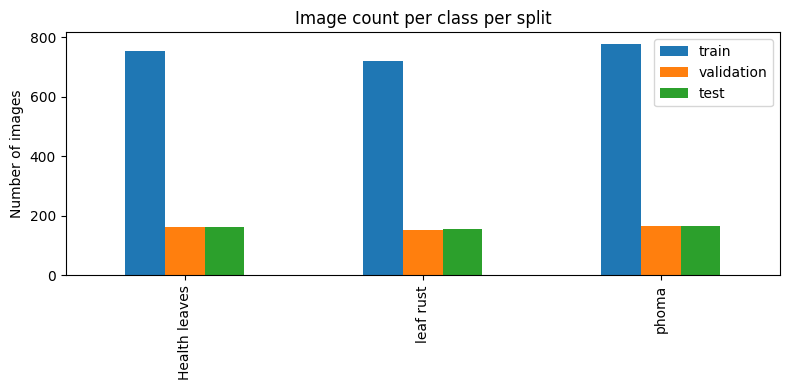
\includegraphics[width=0.95\textwidth]{images/Count of usable images printed by the transfer-learning notebook after image cleansing.png}
\caption{Count of images per class and split after image cleansing.}
\end{figure}

\section{Preprocessing and Experimental Setup}

The images were preprocessed and prepared for training in the same way for all model variants.
The images were read from folders and scaled to 224 x 224 pixels. They were batched with
batch size 32 and transformed to categorical labels. The training set was augmented with
random rotations, width shifts, height shifts, horizontal flips, and zooming. Validation
and test data were not augmented; they were only rescaled.

Models were compiled with categorical cross-entropy as a loss function and Adam optimizer
with the initial learning rate of 0.001. Early stopping, learning-rate reduction on
plateau, and best-model checkpointing were used to reduce overfitting and keep the best
validation model. Finally, the classification reports were generated with scikit-learn using its classification\_report
function \cite{ScikitClassificationReport}.

A methodology limitation was related to the MobileNetV2 preprocessing pipeline. According
to the MobileNetV2 documentation in Keras, rescaling to [0..1] interval was not recommended. The
documentation recommended using the MobileNetV2 preprocessing function to rescale inputs
to [-1..1] interval. Even though the model achieved very good results, its preprocessing
pipeline was not fully aligned with the recommended transfer-learning preprocessing method.

\section{Model 1: MobileNetV2 Transfer Learning}

Model 1 applied MobileNetV2 for feature extraction with transfer learning. Specifically,
MobileNetV2 was proposed as an efficient mobile network with inverted residuals and
linear bottlenecks \cite{Sandler2018}. Similarly, the Keras application guide mentioned that MobileNetV2
applied inverted residual blocks with bottlenecks and supported ImageNet pre-trained
weights \cite{KerasMobileNet}.

The MobileNetV2 base was loaded with ImageNet weights, the original top
classifier was removed, and the base was frozen. The baseline classification head
contained global average pooling, a 0.3 rate dropout, and a dense softmax classifier
with three output classes.
Thus, the workflow matched the typical transfer learning pipeline as follows: loading
pre-trained base model, freezing the base model, creating and stacking the new model on top, and
then training the classifier on the target data \cite{KerasTransferLearning}.

After receiving feedback, an additional MobileNetV2 variant was tested. The original
frozen MobileNetV2 base was kept unchanged, but the classifier head was expanded to give
the model more trainable capacity after feature extraction. The baseline head used
GlobalAverage\allowbreak{}Pooling2D, Dropout(0.3), and a final softmax layer. The improved version
used GlobalAverage\allowbreak{}Pooling2D, followed by Dense(512, relu), batch normalization,
dropout, Dense(256, relu), batch normalization, dropout, and the final three-class
softmax layer. Therefore, the experiment tested whether the pretrained MobileNetV2
features could be used better by a stronger classifier head, without unfreezing the
MobileNetV2 base. In the final comparison, this dense-head variant was treated as Model
3 rather than replacing the baseline MobileNetV2 model.

\begin{table}[ht]
\centering
\small
\renewcommand{\arraystretch}{1.15}
\caption{Architecture comparison between the baseline and dense-head MobileNetV2 variants.}
\begin{tabularx}{\textwidth}{|p{35mm}|X|p{20mm}|p{25mm}|}
\hline
MobileNetV2 version & Classifier head & Frozen base & Trainable parameters \\
\hline
Baseline MobileNetV2 & GAP + Dropout(0.3) + Softmax & Yes & 3,843 \\
Dense-head MobileNetV2 & GAP + Dense(512) + BN + Dropout(0.5) + Dense(256) + BN + Dropout(0.5) + Softmax & Yes & 789,507 \\
\hline
\end{tabularx}
\end{table}

Additionally, an optional fine-tuning stage was included where the top layers of
MobileNetV2 were unfrozen and trained with a reduced learning rate. The results
comparison included the repeated MobileNetV2 baseline score of 94.23\% test accuracy
and the dense-head MobileNetV2 score of 97.53\% test accuracy.

\begin{figure}[ht]
\centering
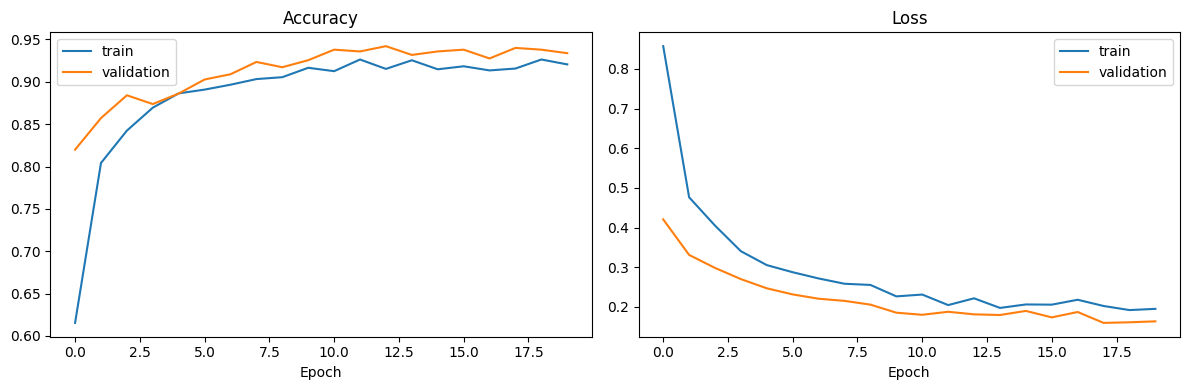
\includegraphics[width=0.95\textwidth]{images/Training and validation accuracy and loss curves for MobileNetV2 with frozen base model.png}
\caption{Training and validation accuracy and loss curves for MobileNetV2 with frozen base model.}
\end{figure}

\section{Model 2: Simple CNN}

Model 2 was a custom convolutional neural network trained from scratch. In contrast to
Model 1, Model 2 did not use pre-trained ImageNet weights. The architecture consisted of
several convolutional blocks with Conv2D layers, batch normalization, max pooling, and
dropout. The last classifier contained dense layers with three class softmax outputs.
Therefore, this design enabled Model 2 to extract features from the coffee leaf images
directly. Still, the training time was longer compared to MobileNetV2 since
all trainable filters needed to be learned from scratch using the project dataset.

\begin{table}[ht]
\centering
\small
\renewcommand{\arraystretch}{1.15}
\caption{Summary of the MobileNetV2 transfer learning model and Simple CNN model.}
\begin{tabularx}{\textwidth}{|p{33mm}|X|X|}
\hline
Component & MobileNetV2 transfer learning model & Simple CNN model \\
\hline
Architecture type & MobileNetV2; include\_top=False; ImageNet weights & Custom CNN trained from scratch \\
Training status & Frozen during the main training run & All model weights trained from the coffee leaf data \\
Layers & GlobalAveragePooling2D; Dropout; Dense layer with 3 softmax outputs & Conv2D, BatchNormalization, MaxPooling2D, Dropout; Dense layer with 3 softmax outputs \\
Total parameters & 2,261,827 & 1,442,851 \\
Trainable parameters & 3,843 & 1,442,851 \\
Number of epochs & 20 epochs & 22 epochs \\
Total training time & ~969 seconds / 16.15 minutes & 4,919.10 seconds / 81.99 minutes \\
\hline
\end{tabularx}
\end{table}

\begin{table}[ht]
\centering
\small
\renewcommand{\arraystretch}{1.15}
\caption{Comparison between the original MobileNetV2 head and the dense-head MobileNetV2.}
\begin{tabularx}{\textwidth}{|p{31mm}|X|X|X|}
\hline
Metric & MobileNetV2 baseline & MobileNetV2 dense head & Better result \\
\hline
Test accuracy & 94.23\% & 97.53\% & Dense-head MobileNetV2 \\
Test loss & 0.1347 & 0.0959 & Dense-head MobileNetV2 \\
Macro-F1 & 0.9423 & 0.9751 & Dense-head MobileNetV2 \\
Total parameters & 2,261,827 & 3,049,027 & Baseline smaller \\
Trainable parameters & 3,843 & 789,507 & Baseline lighter \\
Training time & 14.2 min & 14.2 min & Similar \\
\hline
\end{tabularx}
\end{table}

The training curves demonstrated gradual improvement and slightly unstable validation loss
in the initial training epochs. This was expected for a CNN model trained from scratch due to
randomly initialized network weights. Once the network learned useful visual filters from
the input images, validation accuracy increased, and the model restored the best
performance weights according to the callback settings.

\begin{figure}[ht]
\centering
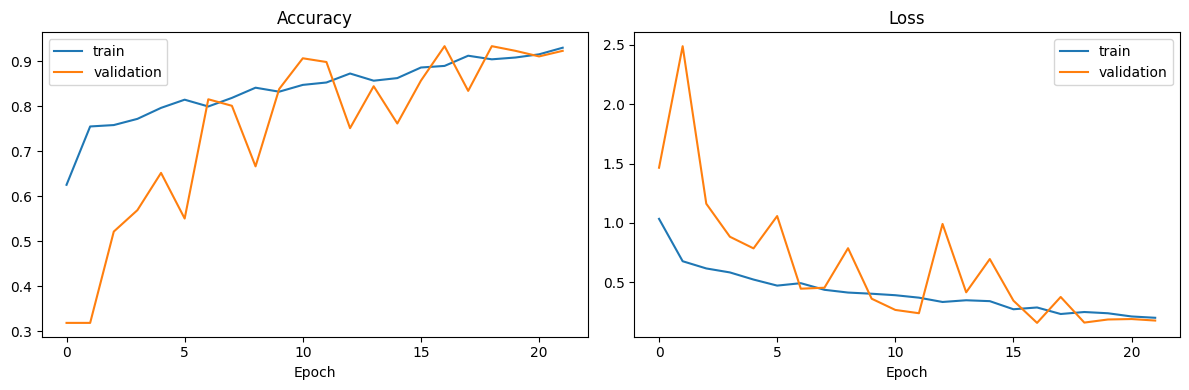
\includegraphics[width=0.95\textwidth]{images/Training and validation accuracy and loss curves for Simple CNN model.png}
\caption{Training and validation accuracy and loss curves for Simple CNN model.}
\end{figure}

\section{Results}

The same hold-out test set of 485 images was used for all model variants. This was an
important criterion for comparability since each model's performance was measured
against the same image distribution and class labels. The additional dense-head
MobileNetV2 experiment was added to test whether the original MobileNetV2 result was
limited by the small classifier head.

\begin{table}[ht]
\centering
\small
\renewcommand{\arraystretch}{1.15}
\caption{General comparison between the MobileNetV2 baseline and Simple CNN based on the experimental outputs.}
\begin{tabularx}{\textwidth}{|p{25mm}|X|X|X|}
\hline
Metric & MobileNetV2 transfer learning & Simple CNN & Best result \\
\hline
Test accuracy & 94.23\% & 95.88\% & Simple CNN \\
Test loss & 0.1347 & 0.1158 & Simple CNN \\
Total parameters & 2,261,827 & 1,442,851 & Simple CNN smaller total model \\
Trainable parameters in main run & 3,843 & 1,442,851 & MobileNetV2 fewer trainable parameters \\
Training time & ~969 seconds / 16.15 minutes & 4,919.10 seconds / 81.99 minutes & MobileNetV2 faster training \\
Training strategy & Transfer learning & From scratch & Depending on objective \\
\hline
\end{tabularx}
\end{table}

A third comparison was added after the professor's feedback. Instead of replacing the
original MobileNetV2 model, a second MobileNetV2 version was trained with a denser
classifier head. This allowed a controlled comparison between two MobileNetV2 variants:
one with a very small classification head and one with additional dense layers copied
from the CNN classifier structure. The dense-head MobileNetV2 achieved 97.53\% test
accuracy, compared with 94.23\% for the MobileNetV2 baseline. This corresponds to an
improvement of 3.30 percentage points. Macro-F1 also increased from 0.9423 to 0.9751,
showing that the improvement was not limited to only one class.

\begin{table}[ht]
\centering
\small
\renewcommand{\arraystretch}{1.15}
\caption{Per-class F1-score comparison between the MobileNetV2 baseline and dense-head MobileNetV2.}
\begin{tabularx}{\textwidth}{|p{35mm}|X|X|X|}
\hline
Class & MobileNetV2 baseline F1 & MobileNetV2 dense-head F1 & Change \\
\hline
Healthy leaves & 0.9657 & 0.9878 & +0.0221 \\
Leaf rust & 0.9221 & 0.9653 & +0.0432 \\
Phoma & 0.9390 & 0.9723 & +0.0333 \\
\hline
\end{tabularx}
\end{table}

\begin{table}[ht]
\centering
\small
\setlength{\tabcolsep}{4pt}
\renewcommand{\arraystretch}{1.15}
\caption{Precision, recall, and F1-score per class in the classification reports.}
\resizebox{\textwidth}{!}{%
\begin{tabular}{|l|r|r|r|r|r|r|}
\hline
Class & MobileNetV2 precision & MobileNetV2 recall & MobileNetV2 F1 & Simple CNN precision & Simple CNN recall & Simple CNN F1 \\
\hline
Healthy leaves & 0.97 & 0.96 & 0.97 & 0.99 & 0.98 & 0.98 \\
Leaf rust & 0.90 & 0.95 & 0.92 & 0.91 & 0.98 & 0.94 \\
Phoma & 0.96 & 0.92 & 0.94 & 0.98 & 0.92 & 0.95 \\
Macro average & 0.94 & 0.94 & 0.94 & 0.96 & 0.96 & 0.96 \\
Weighted average & 0.94 & 0.94 & 0.94 & 0.96 & 0.96 & 0.96 \\
\hline
\end{tabular}
}
\end{table}

\begin{figure}[ht]
\centering
\small
\renewcommand{\arraystretch}{1.15}
\begin{tabular}{|l|r|r|r|}
\hline
True / Predicted & Healthy leaves & Leaf rust & Phoma \\
\hline
Healthy leaves & 155 & 4 & 3 \\
Leaf rust & 4 & 148 & 4 \\
Phoma & 0 & 13 & 154 \\
\hline
\end{tabular}
\caption{Confusion matrix of MobileNetV2 on the test set.}
\end{figure}

\begin{figure}[ht]
\centering
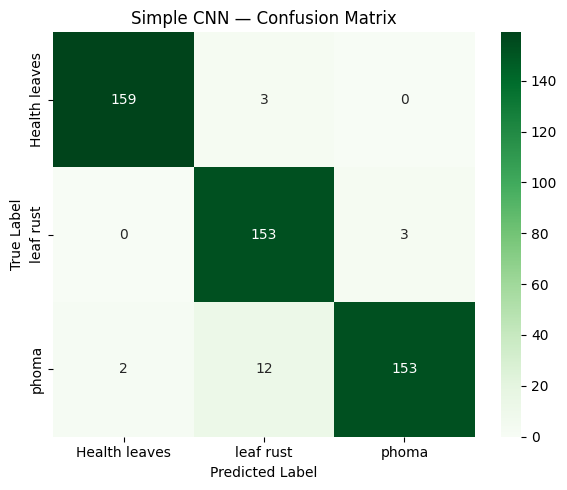
\includegraphics[width=0.65\textwidth]{images/Confusion matrix of Simple CNN on the test set.png}
\caption{Confusion matrix of Simple CNN on the test set.}
\end{figure}

\section{Model Comparison and Discussion}

Before the dense-head MobileNetV2 experiment, the Simple CNN achieved a higher numerical
score than the baseline MobileNetV2, with 95.88\% test accuracy compared to 94.23\%.
However, the dense-head MobileNetV2 then achieved the highest score, with 97.53\% test
accuracy. This suggests that the original MobileNetV2 feature extractor was not
necessarily worse than the Simple CNN; rather, the original classifier head may have been
too small for the final classification task.

The efficiency trade-off also changed after adding the dense head. The baseline
MobileNetV2 had only 3,843 trainable parameters, while the dense-head MobileNetV2 had
789,507 trainable parameters. This was still less than the 1.44 million trainable
parameters in the Simple CNN, but it was much larger than the original MobileNetV2 head.
Therefore, the improved accuracy should be interpreted together with the increased
classifier capacity.

The confusion matrix results showed that healthy leaves were easier for the models to
identify than the two disease classes. The most important remaining confusion was between
Phoma and leaf rust, which is plausible because both disease categories can contain
visually similar spots and lesions on the leaf surface \cite{Esgario2020}.

\begin{figure}[ht]
\centering
\small
\renewcommand{\arraystretch}{1.15}
\begin{tabular}{|l|r|r|r|}
\hline
True / Predicted & Healthy leaves & Leaf rust & Phoma \\
\hline
Healthy leaves & 162 & 0 & 0 \\
Leaf rust & 3 & 153 & 0 \\
Phoma & 1 & 8 & 158 \\
\hline
\end{tabular}
\caption{Confusion matrix of MobileNetV2 with dense classifier head on the test set.}
\end{figure}

The dense-head MobileNetV2 confusion matrix shows that all healthy leaves were
classified correctly. The main remaining error was still between Phoma and leaf rust, but
this error was reduced compared with the baseline MobileNetV2 model. In the baseline
run, 13 Phoma images were predicted as leaf rust, while the dense-head model reduced this
number to 8. This suggests that the additional dense layers improved the separation
between the two visually similar disease classes.

The difference between the baseline MobileNetV2 and Simple CNN was small enough that it
should not be interpreted as final proof that one architecture was always superior.
However, the dense-head MobileNetV2 improved over the baseline by 3.30 percentage
points, which made the classifier-head comparison more informative than the earlier
two-model comparison. A fair final comparison should still include repeating the training
process multiple times, taking the mean and standard deviation of accuracies and macro
F1-scores for all iterations, and ideally including the statistical evaluation of paired
sample predictions.

Another reason that can explain the lower accuracy obtained by the baseline MobileNetV2
could be the use of a non-optimal pre-processing step before training. As stated in the Keras
documentation, mobileNetV2.\allowbreak preprocess\_input must be employed, meaning that the image
pixels' values need to be scaled to [-1, 1]. Moreover, during the process of training
MobileNetV2, most of its layers remained unchanged, meaning that the network did not
fully adjust to the characteristics of the coffee leaf samples.

Keras confirms the MobileNetV2 preprocessing requirement, and its transfer-learning
guide says fine-tuning can improve results but can also overfit if not done carefully
\cite{KerasMobileNetDocumentation2026}.

Finally, care was needed in interpreting the result since the dataset source mentioned
that augmentation techniques were utilized to improve sample diversity \cite{Chelangat2025}. Augmented
versions of the same leaves might have been included in each split, leading to an
overestimated measurement of accuracy. While random training, validation, and test folders
were generated, there was no evidence that the data were split in a manner
that ensured each sample group contained similar augmented variants.

\section{Limitations and Improvements}

The biggest limitations of this experiment are methodological limitations rather than
simply those pertaining to the choice of the model:

\begin{enumerate}
\item MobileNetV2 was not preprocessed optimally. In particular, image rescaling to
[0, 1] range instead of using the standard Keras MobileNetV2 preprocessing function was
done.

\item Fine-tuning of MobileNetV2 was not tested on the test set. As a consequence, it
cannot be concluded definitively how much additional improvement could be obtained by
unfreezing part of the MobileNetV2 base after classifier training.

\item Only one train/validation/test split and one random seed were employed. Repeating
this experiment several times is required in order to confirm whether the dense-head
MobileNetV2 improvement remains stable.

\item The improved MobileNetV2 result was obtained by increasing the number of trainable
parameters in the classifier head from 3,843 to 789,507. Although this improved test
accuracy in the current run, it also increased the risk of overfitting. Therefore, the
result should still be validated by repeating the experiment with several random seeds
and reporting the mean and standard deviation of accuracy and macro-F1.

\item Possible presence of duplicates or augmented images was not considered fully.
Should some images of the same original leaf appear in each of these three sets, the
accuracy of the experiment would be biased.

\item Neither cross-validation nor any external testing was performed. The ability of
these models to recognize diseased leaves on the data from RoCoLe or JMuBEN/JMuBEN2 datasets
must be tested to determine whether the model generalizes outside of the local dataset.

\item Explainability method was omitted. Application of Grad-CAM is required to
ascertain whether the models actually pay attention to the actual signs of disease and
not other factors such as leaf boundaries, backgrounds, or lighting \cite{Selvaraju2017}.
\end{enumerate}

Another improvement is to keep the dense-head MobileNetV2 as a separate third model in
the comparison. This makes the report stronger because it directly answers the feedback
about the simple MobileNetV2 classifier head. The final comparison should therefore
include: Simple CNN, MobileNetV2 baseline, and MobileNetV2 with dense classifier head.

The suggested next experiment is as follows: fix MobileNetV2 preprocessing, test frozen
and fine-tuned versions separately, run all model variants at least five times using
different random seeds, present means and standard deviations for these values, perform
perceptual hashing to detect duplicates, and provide some samples of Grad-CAM output for
classification mistakes.

This problem is known as data leakage. Data leakage leads to overly optimistic results
\cite{Kapoor2023}. Class imbalance negatively impacts CNN's effectiveness in some cases
\cite{Buda2018}.
